% !TeX program = xelatex
\documentclass[UTF8,11pt,a4paper,linespread=1]{ctexart}
\usepackage[margin=26mm]{geometry}
\usepackage{amsmath,amssymb,bm}
\usepackage{setspace}
\setstretch{1.35}
\usepackage{graphicx}
\usepackage[unicode,colorlinks=true,linkcolor=blue]{hyperref}

\begin{document}
\section*{从建模软件导入数据对比图}
\begin{figure}[htbp]
  \centering
  % 把 Python 或 MATLAB 导出的图片放在当前文件夹。
  % 没有图片时显示缺图提示，文档仍能编译。
  \IfFileExists{model_comparison.png}{%
    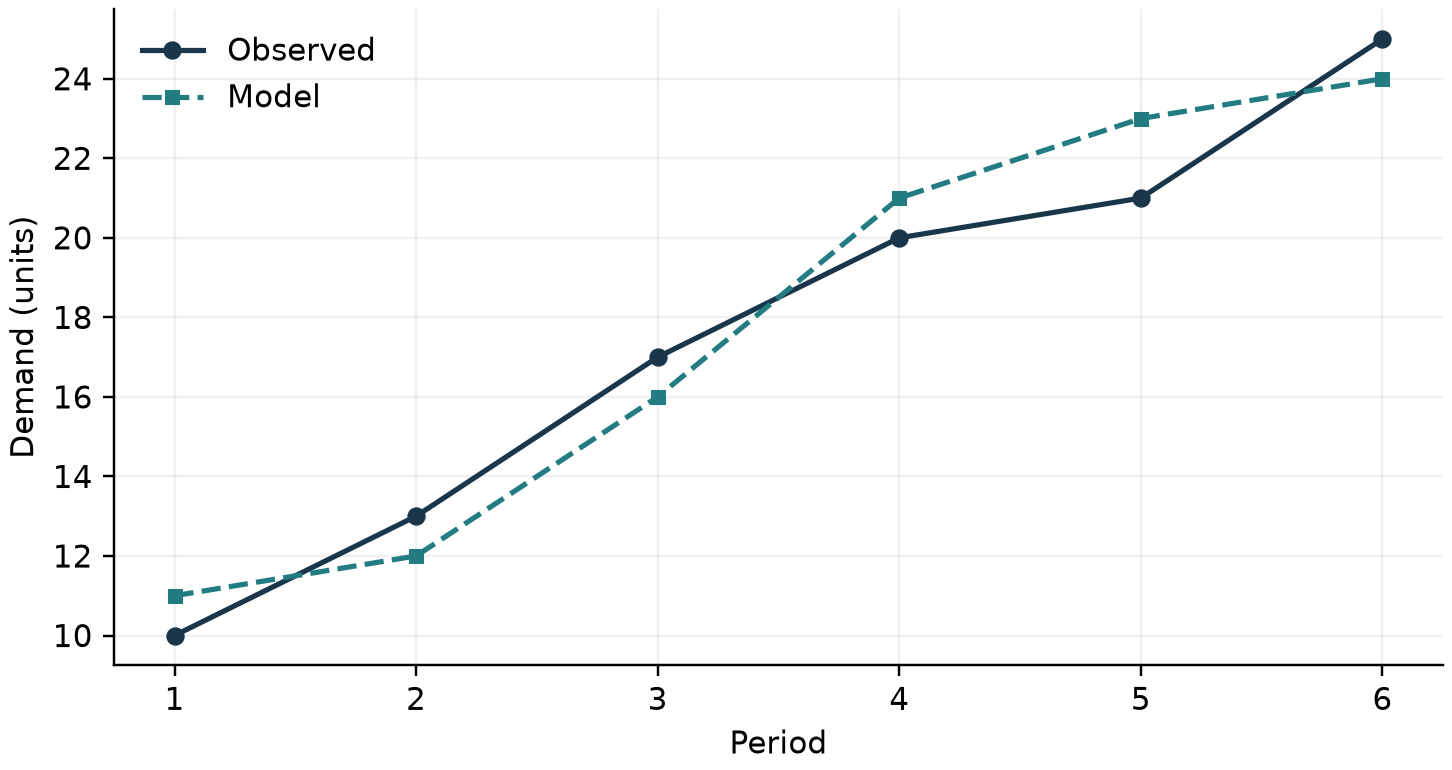
\includegraphics[width=.82\linewidth]{model_comparison.png}
  }{%
    \fbox{\parbox[c][4.5cm][c]{.76\linewidth}{\centering
      未找到数据对比图文件。\\[5pt]
      文件名：model\_comparison.png}}
  }
  \caption{观测值与模型输出的对比；随书数据仅作演示}
  \label{fig:model-comparison}
\end{figure}
图~\ref{fig:model-comparison} 同时标出观测值与模型值，
横纵坐标应写清变量名称和单位。
\end{document}
